\documentclass[11pt,fleqn]{article}

\usepackage[T1]{fontenc}
\usepackage[utf8]{inputenc}
\usepackage[italian]{babel}

\usepackage{graphicx}
\usepackage{amsmath}
\usepackage{amssymb}
\usepackage{bm}

\newcommand{\ul}[1]{\underline{#1}}
\newcommand{\uul}[1]{\ul{\ul{#1}}}

\title{Alcuni chiarimenti}

\begin{document}

\maketitle

\section{Traslazione, rotazione e deformazione e deformazione di un elemento di fluido}
Il moto di un elemento infinitesimo di fluido può essere descritto come composizione di una traslazione, di una rotazione rigida e una deformazione.
Siano $\bm{x}_1(t)$, $\bm{x}_2(t)$ le posizioni di due punti materiali e $\delta\bm{x}(t) = \bm{x}_2(t) - \bm{x}_1(t)$ il vettore che congiunge questi due punti.
La derivata temporale del vettore $\delta \bm{x}(t)$ può essere scritta come
\begin{equation}
 \frac{d \delta\bm{x}}{d t}(t) =
  \frac{d \bm{x}_2}{d t}(t) - \frac{d \bm{x}_1}{d t}(t) = 
  \bm{u}(\bm{x}_2(t),t) - \bm{u}(\bm{x}_1(t),t) \ , 
\end{equation}
avendo sfruttato la definizione di punto materiale per esprimere la sua velocità,
$d \bm{x}_i/dt$, come la velocità del continuo in quel punto, $\bm{u}(\bm{x}_i(t),t)$.
\newline \noindent
Utilizzando la definizione di $\delta \bm{x}(t)$, si può scrivere $\bm{x}_2(t) = \bm{x}_1(t) + \delta \bm{x}(t)$ ed esprimere la velocità calcolata in $\bm{x}_2(t)$ con un'espansione in serie centrata in $\bm{x}_1(t)$,
\begin{equation}
\begin{aligned}
    \bm{u}(\bm{x}_2(t),t) & = \bm{u}(\bm{x}_1(t)+\delta\bm{x}(t),t) = \\
    & = \bm{u}(\bm{x}_1(t),t) + \delta\bm{x}(t) \cdot \bm{\nabla} \bm{u}(\bm{x}_1(t),t) +
    o(|\delta\bm{x}(t)|) \ .
\end{aligned}
\end{equation}
Si può quindi scrivere la derivata temporale di $\delta \bm{x}$ come
\begin{equation}
 \frac{d \delta \bm{x}}{d t}(t) = \delta \bm{x}(t) \cdot \bm{\nabla}\bm{u}(\bm{x}_1(t),t) + o(|\delta\bm{x}(t)|) \ .
\end{equation}
Sfruttando la scomposizione del gradiente della velocità come somma della sua parte simmetrica e della sua parte antisimmetrica, rispettivamente il \textit{tensore velocità di deformazione} $\mathbb{D}$ e \textit{tensore di spin} $\mathbb{R}$, si possono riconoscere i contributi di deformazione e rotazione nell'evoluzione di $\delta \bm{x}(t)$,
\begin{equation}
    \frac{d \delta \bm{x}}{d t}(t) = \delta \bm{x}(t) \cdot \mathbb{D}(\bm{x}_1(t),t) +
                                     \delta \bm{x}(t) \cdot \mathbb{R}(\bm{x}_1(t),t) + o(|\delta\bm{x}(t)|) \ .
\end{equation}
Sfruttando la natura antisimmetrica del tensore di spin $\mathbb{R}$, si può riscrivere il contributo di rotazione al movimento in una forma che dovrebbe essere più familiare (si pensi all'atto di moto rigido, come visto in meccanica razionale)
\begin{equation}
    \frac{d \delta \bm{x}}{d t}(t) = \delta \bm{x}(t) \cdot \mathbb{D}(\bm{x}_1(t),t) + 
    \frac{1}{2} \bm{\omega}(\bm{x}_1(t),t) \times \delta \bm{x}(t) + o(|\delta\bm{x}(t)|) \ ,
\end{equation}
che permette di riconoscere il legame tra vorticità $\bm{\omega}$ e velocità angolare delle particelle materiali: la vorticità $\bm{\omega}(\bm{x},t)$ risulta essere il doppio della velocità angolare della particella materiale che passa per il punto $\bm{x}$ all'istante temporale $t$.
\newline \noindent
L'evoluzione del punto materiale $\bm{x}_2(t)$ può quindi essere espressa in funzione del moto del punto $\bm{x}_1(t)$ e del vettore differenza $\delta\bm{x}_2(t)$,
\begin{equation}
\begin{aligned}
    \frac{d\bm{x}_2}{d t}(t) & = \ \frac{d\bm{x}_1}{d t}(t) + & \text{(traslazione)} \\
    & \ + \frac{1}{2} \bm{\omega}(\bm{x}_1(t),t) \times \delta \bm{x}(t) + & \text{(rotazione)} \\
    & \ + \delta \bm{x}(t) \cdot \mathbb{D}(\bm{x}_1(t),t) + & \text{(deformazione)} \\
    & \ + o(|\delta\bm{x}(t)|) & \text{(termini di ord.sup.)}
\end{aligned}
\end{equation}
riconoscendo i contributi di traslazione, rotazione, deformazione e contributi di ordine superiore che diventano trascurabili per $|\delta\bm{x}(t)| \rightarrow 0$.

\subsection{Esempio: corrente di Newton}
Si considera l'esempio della corrente di Newton in un canale piano infinito, descritta dal campo di velocità 
\begin{equation}
  \bm{u} = \frac{y}{H}U \bm{\hat{x}} \ .
\end{equation}
Si vuole determinare l'evoluzione in un istante di tempo $dt$ di due vettori materiali $\delta \bm{x}_a(t) = \bm{\hat{x}}$, $\delta \bm{x}_b(t) = \bm{\hat{y}}$, per valutare gli effetti di rotazione e deformazione di un volumetto elementare inizialmente quadrato, con i lati orientati come i due vettori considerati.
Si possono raccogliere le componenti cartesiane del gradiente di velocità $\bm{\nabla} \bm{u}$ nella matrice
\begin{equation}
 \left[
 \begin{array}{ccc} 
   u_x & u_y & u_z \\
   v_x & v_y & v_z \\
   w_x & w_y & w_z \\
 \end{array} \right] = 
 \left[
 \begin{array}{ccc} 
   0 & U/H & 0 \\
   0 &  0  & 0 \\
   0 &  0  & 0 \\
 \end{array} \right] \ ,
\end{equation}
e di conseguenza raccogliere le componenti dei tensori $\mathbb{D}$, $\mathbb{R}$ nelle matrici
\begin{equation}
 \uul{D} = 
 \left[
 \begin{array}{ccc} 
   0 & \frac{U}{2H} & 0 \\
   \frac{U}{2H} & 0 & 0 \\
   0 &  0  & 0 \\
 \end{array} \right] \quad , \quad
 \uul{R} = 
 \left[
 \begin{array}{ccc} 
   0 & \frac{U}{2H} & 0 \\
  -\frac{U}{2H} & 0 & 0 \\
   0 &  0  & 0 \\
 \end{array} \right] \ .
\end{equation}
All'istante $t+dt$, le componenti cartesiane $\ul{\delta x_i}(t+dt)$ vettore materiale $\delta \bm{x}_i(t+dt)$ possono essere ricavate come
\begin{equation}
 \begin{aligned}
     \ul{\delta x_i}(t+dt) & = \ul{\delta x_i}(t) + \frac{d \ul{\delta x_i}}{ dt}(t) = \\
     & = \ul{\delta x_i}(t) + \uul{D} \, \ul{\delta x_i} + 
                              \uul{R} \, \ul{\delta x_i} \ .
 \end{aligned}
\end{equation}
Svolgendo i conti per i vettori $\delta \bm{x}_a$, $\delta \bm{x}_b$, si ottiene,
\begin{equation}
 \begin{aligned}
     \ul{\delta x_a}(t+dt) & = \ul{\delta x_a}(t) +
     \left[ \begin{array}{c} 0 \\  \frac{U}{2H} \end{array}  \right] +
     \left[ \begin{array}{c} 0 \\ -\frac{U}{2H} \end{array}  \right] =
     \ul{\delta x_a}(t) =
     \left[ \begin{array}{c} 1 \\ 0 \end{array}  \right]
         \\
     \ul{\delta x_b}(t+dt) & = \ul{\delta x_b}(t) +
     \left[ \begin{array}{c} \frac{U}{2H} \\ 0 \end{array}  \right] +
     \left[ \begin{array}{c} \frac{U}{2H} \\ 0 \end{array}  \right] = 
     \ul{\delta x_a}(t) + 
     \left[ \begin{array}{c} \frac{U}{H} \\ 0 \end{array}  \right] =
     \left[ \begin{array}{c} \frac{U}{H} \\ 1 \end{array}  \right] \ .
 \end{aligned}
\end{equation}
Si può notare che i contributi di rotazione e deformazione sono entrambi non nulli, ma che il loro effetto complessivo si annulla sul vettore $\delta \bm{x}_a$ orientato come la direzione $x$, mentre il loro effetto si somma sul vettore $\delta \bm{x}_b$ inizialmente orientato lungo la direzione $y$, come mostrato in figura.

\begin{center}
 \includegraphics[width=0.95\textwidth]{./rotdef}
\end{center}






\end{document}
